\chapter{Experimenteller Aufbau}
Die Streuung der Röntgenstrahlung an der Probe wird bei den kleinen Winkeln beobachtet. Die Probe im Strahlengang wird \SI{160}{\milli\meter} nach hinten von dem Fokuspunkt der \gls{rzp} gestellt/verschoben. Für die schärfere Abbildung des Streubildes soll der Detektor möglichst nah an der Probe gebracht werden. In der aktuellen Aufbaukonfiguration konnte das dadurch realisiert werden, dass der Detektor an der gegenüberliegenden Wand ca. $l = \SI{607(7)}{\milli\meter}$ von der Probe entfernt befestigt wird.
\begin{figure}[H]
    \centering
    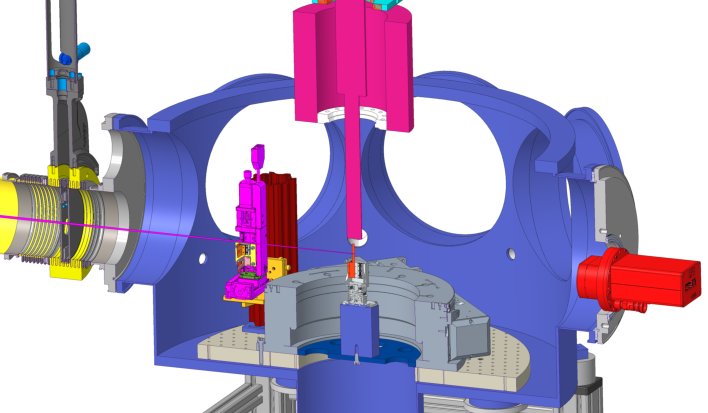
\includegraphics{images/aufbau/aufbau_empty.pdf}
    \caption{Die Skizze des Anlageaufbaus. Die Einzelbauteile sind farbig kodiert. In der Vakuumkammer (blau) wird der Druck in Höhe von ca. \SI{2.4e6}{\milli\bar} aufrechterhaltet. Der Probehalter (pink) lässt sich seitlich bewegen, rotieren und vertikal hoch und herunterfahren. Der horizontale Spalt (fuchsia) dient zum Abschneiden des gewünschten Stahlsanduhrbereichs. Die Spaltlage sowie die Spaltbreite kann beliebig verstellt werden. Der MÖNCH-Detektor (rot) ist an der zum Strahlgang (gelb) gegenüberliegenden Wand der Vakuumkammer befestigt.}
    \label{fig:anlage}
\end{figure}
\noindent
Die Messungen wurden im Rahmen dieser Arbeit lediglich an der Photonenenergie $h\nu_\text{Gd, M5}$ durchgeführt, weil der \gls{adu}-Wert pro ein Photon bei dieser Photonenenergie fast doppelt so hoch ist, als bei der Photonenenergie $h\nu_\text{Fe, L3}$, was im Endeffekt das ursprüngliche \gls{snr} erhöht und die potenziell bessere Ergebnisse nach der Auswertung gewährleisten soll.

% \noindent
% In der ersten Näherung kann die Domänenstruktur der Probe \textbf{DS220126} als ein Gitter betrachtet werden, wobei die Domänengröße dem Spaltabstand $d$ entspricht. Dieser kann mit den MFM-Aufnahmen (Abb. \ref{fig:mfm-amplitude-ft}c)) mit ca. \SI{300}{\nano\meter} abgeschätzt werden. In Hinblick darauf, dass die Streuung in der aktuellen Transmissionsgeometrie unter den kleinen Winkeln beobachtet wird, lässt sich der Abstand des $k$-ten Maximums zum $0$-ten Maximum wie folgt ermitteln
% \begin{equation}
%      r_{k} = \frac{kl\lambda}{d},
%  \end{equation}
%  wobei $l = \SI{607(6)}{\milli\meter}$ - Abstand vom Gitter bis zur Beobachtungsfläche und $\lambda$ - Photonenwellenlänge. Die Photonenenergie $h\nu_{\text{Gd, M5}} = \SI{1184,79}{\eV}$ entspricht der Wellenlänge $\lambda_{\text{Gd, M5}} = \SI{1,05}{\nano\meter}$. So ist der erwartete Abstand des 1. Streuringes bis zum $0$-ten Hauptmaxima 
%  \begin{equation}
%      r_{1, \text{ Gd, M5}} = \frac{1 \cdot l\lambda_{\text{Gd, M5}}}{d} = \SI{2.12(2)}{\milli\meter}.
%      \label{eq:theo_r1}
% \end{equation}
\noindent
Die Dunkelbilder, die nachher aus den Aufnahmen subtrahiert werden (s. Abschnitt \ref{text:moench_theorie}), werden jede 30 Minuten in Höhe von \num{10000} Stück aufgenommen, um die zeitliche Entwicklung des Hintergrundrauschens mitzunehmen. Ein kontinuierlicher Aufnahmevorgang der \gls{pxs} kann höchstens bis \SI{20}{\second} dauern. Die Pulsfrequenz $f_\text{\gls{pxs}}$ ist konstant und beträgt \SI{100}{\hertz}. So werden es \num{2000} Pulsen innerhalb eines \SI{20}{\second} Aufnahmevorgangs emittiert. Jedem Puls geht ein Triggersignal voraus, das \SI{1}{\milli\second} vor dem Puls generiert wird.

\noindent
Der \gls{moench03} hat eine einstellbare Verzögerung zwischen dem Aufnahmestart und dem Trigersignaleingang. Diese wird so konfiguriert, dass der \SI{10}{\femto\second} Röntgen-Puls der \gls{pxs} innerhalb des Belichtungszeitfensters $\tau$ vollständig/komplett hineinpasst. So könne die Belichtungszeit theoretisch weit bis dieselbe Großenordnung wie Pulslänge gesenkt. Das konnte aber praktisch nicht realisiert werden, weil die resultierende zeitliche Schwankung des Triggersignal-Generators, inneren Taktieren von \gls{moench03} Dutzende von \si{\nano\second} beträgt. So konnte die Belichtungszeit $\tau$ unter der Bedingung, dass jeder Puls komplett in jeder Aufnahme aufgenommen wird, höchstens bis auf \SI{1}{\micro\second} heruntergesetzt werden.

\noindent
Durch die Verkleinerung der Spalthöhe lässt sich ein kleinerer Energiebereich um die Resonanzenergie, der auf die Probe abgebildet wird, selektieren und die nichtresonanten Energien abschneiden, wodurch die Überlagerung des Direktstahls mit dem Streuring vermieden werden kann und die bessere Energieauflösung erreichbar ist. Die Beugung an den Spaltkanten kann sich jedoch mit der Beugung an der Probe überlagern und nicht davon trennbar sein. Aus diesem Grund wurden die Messungen sowohl mit dem schmal eingestellten Spalt als auch ohne den Spalt durchgeführt

\noindent
Neben der Strahlung im Röntgenspektrum tritt bei der \gls{pxs} auch Strahlung im sichtbaren Spektrum, Streuung des einfallenden Laserlichts und Elektronenemission auf. Obwohl der Sensor von \gls{moench03} \SI{500}{\nano\meter} Al-Beschichtung habe, scheint sie am Rande dünner zu sein. So wurden die Pixel am Rande des Detektors ständig belichtet, selbst wenn der Röntgenstrahl in großer Entfernung von dem Sensorrand projiziert wurde. Es wurde daher zusätzlich im Strahlgang eine Mylar Folie mit \SI{200}{\nano\meter} Al-Beschichtung installiert, die die Intensität des sichtbaren und infraroten Lichtes deutlich abschwächte und dadurch den beobachteten Halo-Effekt beseitigte. Obwohl die Elektronen mit einem starken Magnet von dem Strahlgang großenteils abgelenkt werden, konnten einigen Elektronen auf dem \gls{moench03} detektiert werden. Der installierte Filter reduzierte ihre Zahl auch.
%
% \noindent
% Könnte die Belichtungszeit $\tau$ auf \SI{100}{\nano\second} gesetzt werden, ließ sich die Standardabweichung $\sigma$ von ca. \SI{21}{\adu} bis \SI{19}{\adu} senken. So würde das ursprüngliche \gls{snr} immer noch im Bereich von 7-\SI{10}{\decibel} liegen.

\noindent
Der Streuungseffekt der Proben ist energieselektiv und tritt am stärksten nur im schmalen Bereich um der Resonanzenergie $h\nu_{\text{Fe, L3}}$ bzw. $h\nu_{\text{Gd, M5}}$ auf. Diese Energien sind die weder Zielenergien von \gls{rzp} für Fe, noch für Gd. Aus diesem Grund muss der Strahl mit dem Fokuspunkt horizontal verschoben werden, damit die Resonanzenergie mittig an dem Detektor liegt und auf die Probe projiziert werden kann. Die Effizienz und die Abbildungsschärfe der \gls{rzp}, also die Energieauflösung pro Längeeinheit entlang der Energieachse, sind jedoch maximal an der Zielenergie und nehmen ständig mit der Entfernung von der Zielenergie ab.

\noindent
Im Abschnitt \ref{text:quelle_roentgen} wurde der detektierte Photonenfluss ohne Probe von \gls{pxs} angegeben. In Hinblick auf die niedrige erwartete Transsmissionsrate der Probe \textbf{DS220126} (Abb. \ref{fig:proben_vergleich_centered}) wurde der Photonenfluss, der schließlich nach der Streuung an der Probe detektiert wird, erneut experimentell bestimmt. Dieses Verfahren ist in Unterabschnitt \ref{text:streuung_counting} detalliert präsentiert.

\noindent
Der detektierte Photonenfluss mit der Probe konnte mit \SI{60(5)}{\photons} pro Puls abgeschätzt werden, wobei ca. \SI{45(5)}{\photons} in dem Direktstrahl liegen. Es werden insgesamt \numrange{40000}{50000} Pulsen aufgenommen, damit Kontrast und Schärfe im Maximabereich 1. Ordnung vom Streumuster ausreichend sind. 
% Die Streuung an der gegebenen Probe kann in erster Näherung als die Streuung an einem Gitter betrachtet werden. So ist die Intensitätsverteilung
% \begin{equation}
%     I(r, \varphi) \propto \sinc^2(R),
% \end{equation}
% wobei $r$ - Entfernung (Radius) vom Zentrum des Streubildes.

% \noindent
% So ist die gesamte Intensität innerhalb der 0. Ordnung
% \begin{equation}
%     I_{0. \text{Ordnung}} = \int_{0}^{2\pi}\int_{0}^{\pi}r\sinc^2(r) dr d\varphi \approx \num{7.66} 
% \end{equation}
% und 1. Ordnung
% \begin{equation}
%     I_{1. \text{Ordnung}} = \int_{0}^{2\pi}\int_{\pi}^{2\pi}r\sinc^2(r) dr d\varphi \approx \num{2.13} 
% \end{equation}
% Die Fläche sind jeweils
% \begin{equation}
%     A_{0. \text{Ordnung}} = \int_{0}^{2\pi}\int_{0}^{\pi}rdr d\varphi = \pi^3
% \end{equation}
% und
% \begin{equation}
%     A_{1. \text{Ordnung}} = \int_{0}^{2\pi}\int_{\pi}^{2\pi}rdr d\varphi = 3\pi^3
% \end{equation}
% D.h., dass die Intensitätdichten $\rho$
% sind
% \begin{equation}
%     \rho_{N. \text{Ordnung}} = \frac{I_{N. \text{Ordnung}}}{A_{N.}}
% \end{equation}
% \noindent
% Also
% \begin{equation}
%     \rho_{0. \text{Ordnung}}:\rho_{1. \text{Ordnung}} =  \frac{I_{0. \text{Ordnung}}}{A_{0. \text{Ordnung}}} : \frac{I_{1. \text{Ordnung}}}{A_{1. \text{Ordnung}}}   \approx 10:1
% \end{equation}
% Der erwartete Radius des Streuringes (1. Ordnung) kann mit der Formel für ein Gitter mit Kleinwinkelnäherung
% \begin{equation}
%     a_k = \frac{kl\lambda}{d},
% \end{equation}
% wobei $k$ - Ordnung des Maximums, $l$ - Abstand vom Gitter bis zum Detektor, $\lambda$ - Photonenwellenlänge und $d$ - Domänengröße. Die Photonenenergie $h\nu_{\text{Gd, M5}} = \SI{1184,79}{\eV}$ entspricht der Wellenlänge $\lambda_{\text{Gd, M5}} = \SI{1,05}{\nano\meter}$. So ist der erwartete Radius für die $h\nu_{\text{Gd, M5}}$ beträgt
% \begin{equation}
%     r_{\text{Gd, M5}} = \frac{kl\lambda_{\text{Gd, M5}}}{d} = \frac{1\cdot\SI{620}{\milli\meter}\cdot\SI{1,05}{\nano\meter}}{\SI{300}{\nano\meter}} = \SI{2.17}{\milli\meter}
% \end{equation}
% Mit der bekannten Auflösung von \gls{moench03}, die \SI{400}{\px}x\SI{400}{\px} ist, und der bekannten Sensorgröße \SI{10}{\milli\meter}x\SI{10}{\milli\meter} kann dieser Wert kann in die Pixel umgerechnet werden
% \begin{equation}
%         r_{\text{Gd, M5}} = \SI{2.17}{\milli\meter} = \frac{\SI{400}{\px}}{\SI{10}{\milli\meter}}\SI{2.1}{\milli\meter}=\SI{87(1)}{\px}
% \end{equation}
% \noindent
% Das entspricht dem 1. Maximum von $\sinc(r)^2$ an der Stelle $r=\SI{4.49}{}$. So ist die Proporitonalität zwischen der ursprünglichen $\sinc(r)^2$ und den tatsächlichen gefunden und beträgt 
% \begin{equation}
%     c_0 = \frac{\SI{87}{\px}}{\num{4.49}} = \SI{19.37}{\px}
% \end{equation}

% \noindent
% So entsprechen den Werten $r=\pi;2\pi$ vom Beugungsminima die Werte
% \begin{equation}
%     r_\text{0. px} = \pi\cdot \SI{19.37}{\px} = \SI{61}{\px}
% \end{equation}
% \begin{equation}
%     r_\text{0. px} = 2\pi\cdot \SI{19.37}{\px} = \SI{122}{\px}
% \end{equation}
% Die Flächen werden dann analog dazu umgerechnet

% \begin{equation}
%     A_{0.} = \pi\cdot (\SI{61(1)}{\px})^2 = \SI{1.2e4}{\px\squared}
% \end{equation}
% \begin{equation}
%     A_{1.} = 3\pi\cdot (\SI{122(1)}{px})^2 = \SI{1.4e5}{\px\squared}
% \end{equation}
% Wir haben tatsächlich \SI{30}{\photons} in $A_{0.}$ pro ein Schuss. So ist die
% \begin{equation}
%     \rho_0 = \frac{\SI{30}{\photons}}{\SI{1.2e4}{\px\squared}} = \SI{2.5e-3}{\photons\per\px\squared}
% \end{equation}
% Für die 1. Ordnung ist das eben dann 10 mal kleiner
% \begin{equation}
%     \rho_1 = \frac{\rho_0}{10} =  \SI{2.5e-4}{\photons\per\px\squared}
% \end{equation}
% Also wollen wir die dichte \SI{1}{\photon\per\px\squared} in dem Ring haben, dann muss man
% \begin{equation}
%     N = \frac{1}{\SI{2.5e-4}{\photons\per\px\squared pro Schuss}} = \SI{4000}{Sch"usse}
% \end{equation}
% machen.
%\cite[„Supplementary information“]{pfau_ultrafast_2012}